\chapter{Implementacja}
\section{Projekt w Unity}
\subsection{Graficzny interfejs użytkownika}
W momencie rozpoczynania prac nad aplikacją Unity w wersji 4.6 było jeszcze w fazie testów beta. Zdecydowałyśmy się jednak na jego użycie, gdyż wprowadzony został w nim bardzo istotny element – nowy silnik do tworzenia interfejsu użytkownika. Tworzenie elementów w starym silniku wymagało deklarowania ich bezpośrednio w kodzie, bez możliwości podglądu widoku zanim projekt nie został skompilowany i uruchomiony. Dodatkowo wszelką obsługę zmiany rozdzielczości i skalowania elementów również należało zaimplementować we własnym zakresie. A nie jest to proste, szczególnie w przypadku aplikacji tworzonych na urządzenia mobilne, które posiadają bardzo zróżnicowane rozdzielczości ekranów.

\begin{figure*}[htbp]
    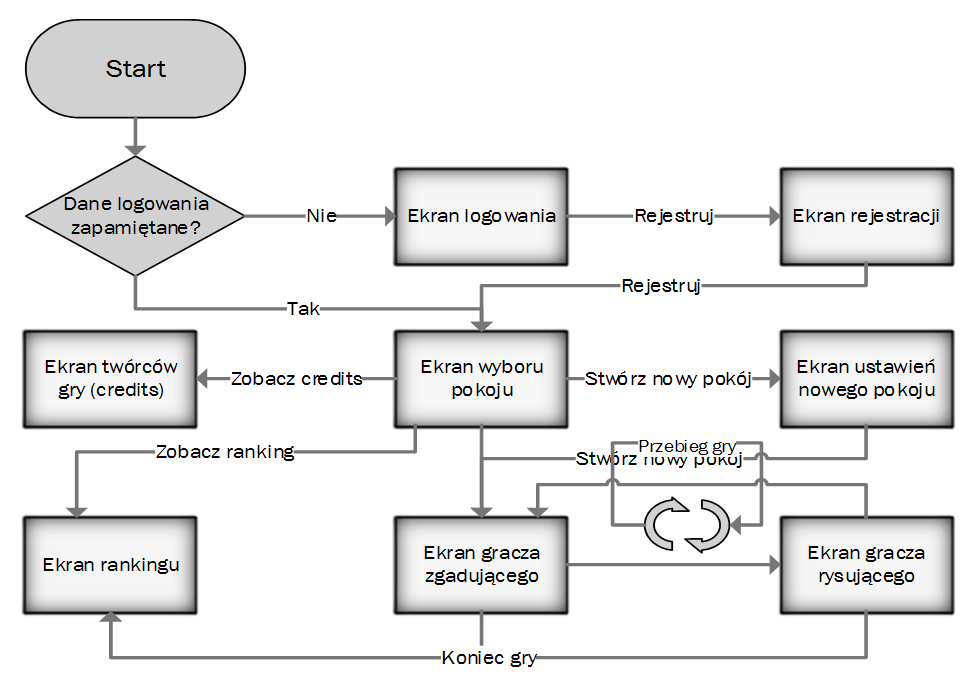
\includegraphics[width=\textwidth]{Flow}
    \caption{Przejścia między ekranami.}
    \label{fig:flow}
\end{figure*}

W nowej wersji silnika sposób tworzenia graficznego interfejsu użytkownika przypomina bardziej ten znany z takich technologii jak na przykład WPF (Windows Presentation Foundation) czy WinForms – możliwe jest manualne ustawianie i zmiana rozmiaru elementów. Dodatkowo, każdy element ma przypisane tzw. punkty zakotwiczenia (ang. anchors), które służą do ustalenia wymiarów i pozycji relatywnie do rozmiaru elementu nadrzędnego. Znacznie ułatwiło to tworzenie naszej aplikacji. Rysunek \ref{fig:flow} przedstawia przejścia między ekranami w Sculpicu.

\subsection{Rozgrywka}
\begin{figure}[htbp]
    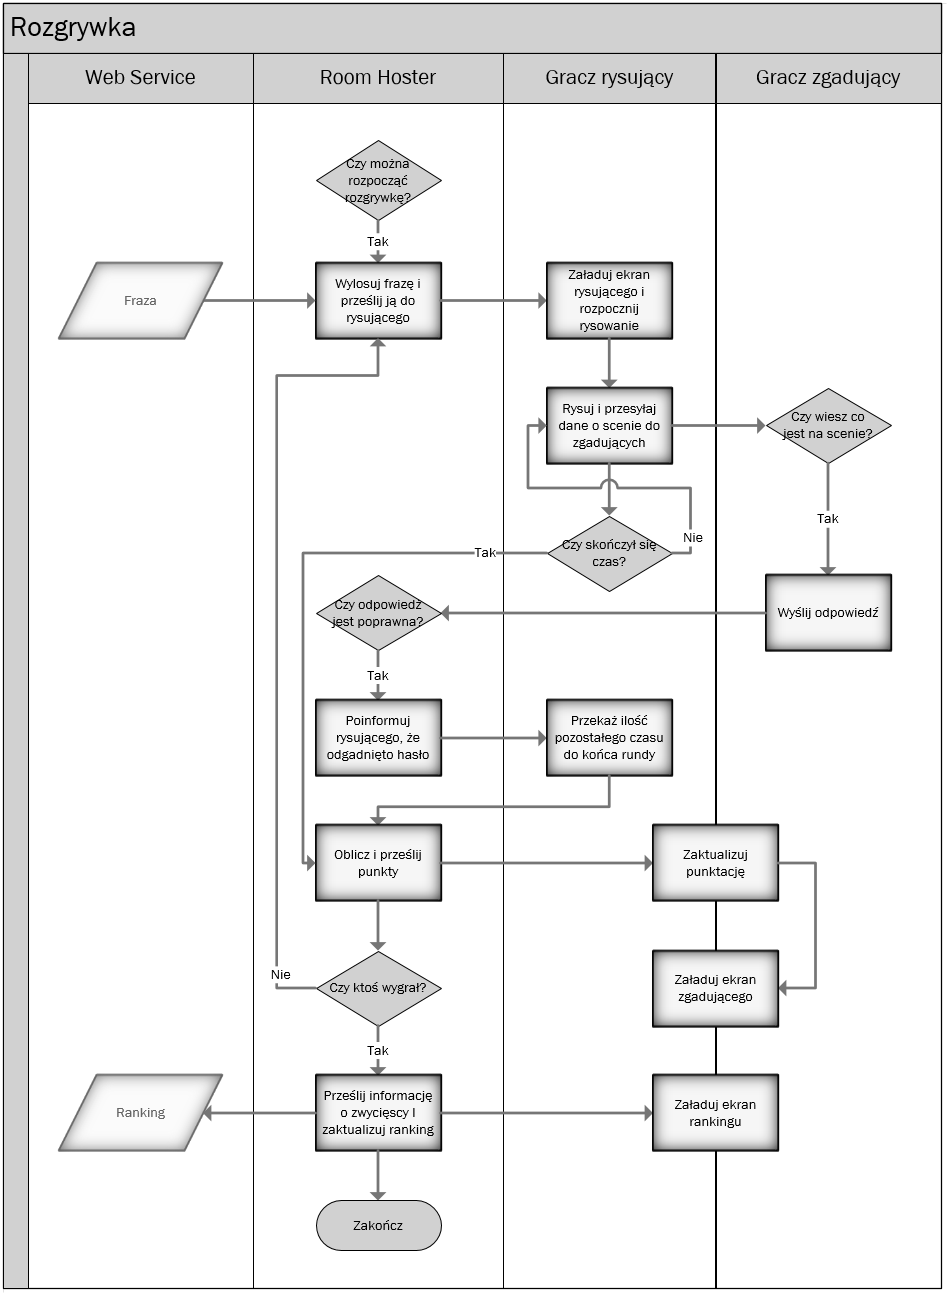
\includegraphics[width=\textwidth]{Gameplay}
    \caption{Diagram przedstawiający rozgrywkę.}
    \label{fig:gameplay}
\end{figure}

Po włączeniu klienta gry i zalogowaniu się, użytkownik może dołączyć do pokoju lub założyć nowy. Gdy użytkownik dołączy do pokoju, do wszystkich graczy znajdujących się w danym pokoju rozsyłana jest informacja o nowej osobie w pokoju. U każdego z nich aktualizowana jest lista aktualnie podłączonych graczy. Aplikacja ładuje wtedy ekran gracza zgadującego.

By rozgrywka się rozpoczęła muszą zostać spełnione 2 warunki:
\begin{enumerate}
    \item w pokoju muszą się znajdować co najmniej 2 osoby,
    \item co najmniej jedna osoba musi się zapisać do kolejki osób rysujących poprzez zaznaczenie opcji \textit{I want to draw}.
\end{enumerate}

Sposób, w jaki odbywa się rozgrywka jest widoczny na rysunku \ref{fig:gameplay}. Wyróżniamy podczas niej kilka ważnych elementów opisanych poniżej.

\subsubsection{Obsługa kolejki graczy chcących rysować}
Odbywa się to w następujący sposób:
\begin{enumerate}
    \item Z kolejki graczy chcących rysować zdejmowany jest pierwszy gracz.
    \item Wysyłana jest do niego fraza, którą ma rysować.
    \item Po zakończeniu rysowania gracz jest ponownie umieszczany w kolejce graczy chcących rysować.
\end{enumerate}

\subsubsection{Hasło do zgadnięcia}
Fraza jest losowana, gdy wiadomo już, że gra może się rozpocząć. Odbywa się to poprzez wywołanie zapytania z Web Service'u. Następnie hasło jest wysyłane do gracza, który ma w tej rundzie rysować. Od tego momentu, wszystkie wiadomości w chacie są sprawdzane po stronie Room Hostera pod kątem zgodności z rysowanym hasłem. Gdy wynik jest pozytywny, ogłaszany jest zwycięsca rundy.

\subsubsection{Czas}
Podczas rundy gracz ma ogrniczony czas, w którym może rysować. Gdy ten czas się skończy, gracz otrzymuje ujemne punkty i wybierana jest kolejna osoba do rysowania (procedura jest taka sama jak przy zgadnięciu, z tą różnicą, że nikt nie zdobywa dodatnich punktów).

\subsubsection{Koniec gry}
Podczas całej rozgrywki Room Hoster po zakończeniu każdej rundy rozsyła graczom punkty, o jakie powinni zaktualizować swoją lokalną punktację. Po stronie Room Hostera ta punktacja jest aktualizowana w taki sam sposób. Dzięki temu możliwe jest śledzenie, czy któryś z graczy nie osiągnął odpowiedniej ilości punktów, by zakończyć grę. Tym samym zapewniamy, że niemożliwe jest oszukanie gry w kwestii punktów, ponieważ są one niezależnie liczone przez aplikację znajdującą się na serwerze. Gdy pułap zostanie osiągnięty, Room Hoster informuje o końcu gry wszystkich graczy, a sam wysyła do Web Service'u informację o aktualizacji rankingów graczy, którzy brali udział w danej rozgrywce.

\subsection{Dotyk}
W grze zaimplementowana została obsługa dotyku na urządzeniach mobilnych. Jest ona wykorzystywana do:
\begin{enumerate}
	\item obracania kamery wokół środka sceny (dostępne dla rysującego i zgadującego),
	\item przesuwania obiektów po scenie (dostępne dla rysującego).
\end{enumerate}

\subsection{Punktacja}
Po wygraniu każdej rundy graczom przydzielane są punkty w zależności od ilości czasu, który upłynął od rozpoczęcia rysowania, odpowiednio:
\begin{itemize}
    \item do 1 minuty – maksymalna ilość punktów,
    \item od 1 minut do 2 minut – 4/5 maksymalnej ilości punktów,
    \item od 2 minut do 3 minut – 3/5 maksymalnej ilości punktów,
    \item od 3 minut do 4 minut – 2/5 maksymalnej ilości punktów,
    \item od 4 minut do 5 minut – 1/5 maksymalnej ilości punktów,
\end{itemize}
Maksymalna ilość punktów wynosi:
\begin{itemize}
    \item 20 dla gracza zgadującego,
    \item 30 dla gracza rysującego.
\end{itemize}

\subsection{Komunikacja}
Najpowszechniejszymi sposobami komunikacji w naszym projekcie są zapytania REST oraz zdalne wywołania procedur (RPC - Remote Procedure Call) zapewnione przez Unity i Master Server. 
Komunikacja z serwerem bazodanowym zostanie opisana w kolejnym podrozdziale, teraz opiszemy komunikację przy pomocy RPC.

\subsubsection{Remote Procedure Calls}
Unity daje możliwość oznaczenia wybranych metod atrubutem [RPC]. Dzięki temu możemy wywoływać taką metodę na odpowiadającym obiekcie w innej aplikacji klienckiej. Istnieje kilka warunków, które należy spełnić, by uzyskać oczekiwany efekt.
\begin{enumerate}
    \item Obiekt deklarujący metody RPC musi mieć podłączony do siebie komponent NetworkView (z przestrzeni nazw UnityEngine).
    \item Metoda może mieć argumenty jedynie określonych typów (szczegóły znajdują się w dokumentacji Unity).
    \item Wszystkie obiekty (ten, który wywołuje oraz te, na których metoda jest wywoływana) muszą mieć wywoływaną metodę zadeklarowaną. Nawet jeżeli miałaby ona nie mieć wnętrza.
\end{enumerate}

\subsubsection{Master Server}
Działanie RPC zapewnione jest za pośrednictwem Master Servera. Unity Technologies udostępniają instancję tej aplikacji użytku programistów Unity. Jednak o wiele wygodniej, co też czynimy w naszym projekcie, jest wykorzystać dostępny kod źródłowy MasterServera dostarczony przez Unity Technologies, by zbudować i włączyć własną instancję owej aplikacji. Ma to wiele zalet, co najważniejsze – posiadamy władzę nad jej czasem działania i nie jesteśmy zależne od dostępności bardzo istotnego w naszym projekcie komponentu.

\subsection{Pokój}
Pokój jest reprezentowany przez aplikację Room Hoster. Zawiera ona całą, wcześniej opisaną funkcjonalność. Najważniejszym skryptem w niej umieszonym jest Room. Znajdujące się tam metody mają za zadanie czuwać nad prawidłowym działaniem komponentów pokoju – kolejką graczy chcących rysować, początkiem i końcem rundy oraz gry, przydzielaniem punktów po każdej rundzie i aktualizacją rankingu.

\section{Serwer bazodanowy}
Na serwer komunikujący się z bazą danych składają się trzy projekty:
\begin{enumerate}
    \item Database – biblioteka do łączenia się z bazą danych, wraz z implementacją dla bazy MongoDB,
    \item WcfServer – zawiera implementację serwisów oraz repozytoriów,
    \item ServerHost – aplikacja konsolowa hostująca usługi WCF.
\end{enumerate}

\subsection{Dostęp do bazy danych}
 
\begin{figure}[htbp]
\centering
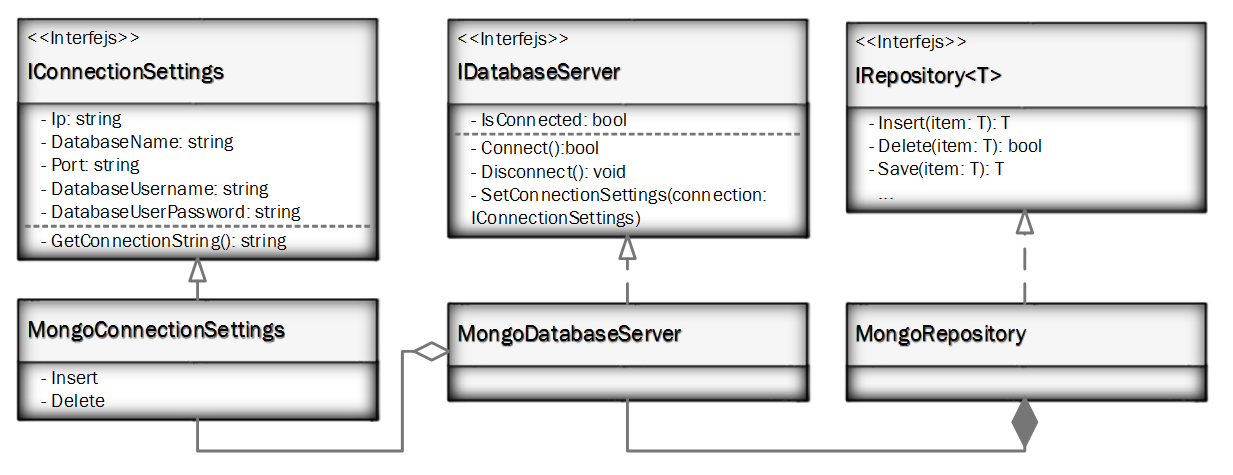
\includegraphics[width=\textwidth]{Database}
\caption{Schemat biblioteki do dostępu do bazy danych.}
\label{fig:database}
\end{figure}
 
Biblioteka przedstawiona na rysunku \ref{fig:database} zawiera podstawowe interfejsy niezbędne do komunikacji z bazą danych, takie jak:
\begin{itemize}
\item IConnectionSettings – model ustawień bazy danych, zawiera informacje dotyczące serwera: IP, port, nazwa bazy danych, użytkownik i hasło; definiuje również metodę GetConnectionString;
\item IDatabaseServer – zawiera podstawowe metody niezbędne przy współpracy z bazą danych umożliwiające połączenie, rozłączenie, zmianę ustawień oraz sprawdzenie, czy połączenie jest aktywne;
\item IRepository<T> - definiuje operacje możliwe do przeprowadzenia na danych, takie jak wstawienie rekordu bądź wywołanie zapytania.
\end{itemize}

Dzięki użyciu w aplikacji interfejsów zamiast konkretnej implementacji możliwe jest łatwe dodawanie obsługi nowego rodzaju bazy danych. Ich użycie jest również szczególnie przydatne w przypadku, gdy aplikacja korzysta z kontenera IoC. W biblioteczce znajduje się również implementacja wyżej wymienionych interfejsów przy użyciu sterownika Mongo C{\#} Driver.

\subsection{Serwer WCF}
W tym projekcie znajduje się implementacja serwisów wykorzystywanych przez klienta gry do zarządzania użytkownikami, losowania haseł oraz tworzenia pokojów. Zawiera on też dodatkowe metody potrzebne do komunikacji z bazą danych w postaci repozytoriów. Usługi stworzone są w architekturze REST, zapytania wywoływane są metodą GET, formatem odpowiedzi jest JSON.

\subsubsection{Zarządzanie użytkownikami}
Usługi umożliwiające zarządzanie użytkownikami znajdują się w klasie UserService, z którą powiązany jest model User oraz repozytorium UserRepository. Do najważniejszych jej metod należą:
\begin{itemize}
\item LoginUser – umożliwia zalogowanie użytkownika, na podstawie podanego loginu i hasła zwracane są dane użytkownika; ponadto w bazie zapisywana jest data ostatniego logowania;
\item AddNewUser – służy do rejestracji nowych użytkowników;
\item PingService – metoda nie przyjmuje żadnych argumentów i zwraca jedynie informację o powodzeniu nawiązania połączenia z serwisem; wywoływana jest przy starcie aplikacji klienckiej w celu rozwiązania adresu IP domeny, dzięki czemu kolejne zapytania wykonywane są dużo szybciej.
\end{itemize}

\subsubsection{Ranking}
Pozycja graczy w rankingu Sculpica jest określana podobnie jak w rankingu szachistów – wykorzystałyśmy metodę obliczania relatywnej siły graczy w punktacji elo. Jednak w przypadku gry wieloosobowej potrzebna była modyfikacja tego systemu, gdyż elo uwzględnia jedynie pojedynki dwóch graczy. Dlatego też każda grupowa gra w Sculpica jest uznawana jako wiele gier jeden na jeden (jakby każdy gracz odbył grę z każdym). W ten sposób do rankingu każdego gracza uczestniczącego w grze dodawana jest suma różnic w rankingu uzyskanych przy obliczeniach dla poszczególnych par.

Aktualizacja rankingu odbywa się poprzez wywołanie metody UpdateRanking w UserService. Jako argumenty podaje się dwa ciągi znaków:
\begin{enumerate}
    \item nazwy użytkowników oddzielone średnikami,
    \item odpowiadające użytkownikom punkty zdobyte podczas rozgrywki oddzielone średnikami.
\end{enumerate}
Metoda ta wykorzystuje klasię EloRanking, w której zawarłyśmy logikę obliczania rankingu.

\paragraph{Obliczanie rankingu}
Dla gracza $X$ o rankingu $R_X$, który grał z graczem $Y$ o rankingu $R_Y$ najpierw obliczana jest różnica rankingów obu graczy:
$dR=R_Y-R_X$.

Następnie oczekiwany wynik rozgrywki, który zawiera się w zakresie $<0,1>$ (gdzie $0$ oznacza przegraną gracza $X$, $0,5$ – remis, a $1$ – przegraną gracza $X$):

\begin{center}
$\displaystyle{\mu S = {{1} \over {(1+10^(dR/400))}}}$.
\end{center}

Przez $S$ oznaczymy rzeczywisty wynik rozgrywki (przyjmuje on wartość według przedstawionych powyżej zasad. Wykorzystamy go do obliczenia różnicy między wynikiem oczekiwanym a rzeczywistym: $dS=S-\mu S$.

Ostatecznie zmiana w rankingu gracza $X$ $dR_X$ wynosi: $dR_X=R_Y+(K*dS)$

Za stałą $K$ przyjęłyśmy liczbę $32$. Niezależnie od początkowego rankingu graczy, w \textit{Sculpicu} stała ta jest taka sama. W ogólnym przypadku można wykorzystać tę stałą do kontrolowania tempa zmian rankingu w zależności od jego wartości.

\subsubsection{Losowanie frazy do odgadnięcia}
Serwisem służącym do pobrania hasła z bazy jest PhraseService z metodą DrawPhrase. Hasła w bazie przechowywane są w postaci modelu Phrase, w którym oprócz samego hasła znajdują się też takie informacje jak ilość wylosowań oraz losowa liczba, służąca do optymalizacji zapytania losującego hasło z bazy.

Z tym serwisem związane jest repozytorium PhraseService, które zawiera tylko jedną metodę – GetRandomPhrase. Najbardziej oczywistym podejściem do losowania hasła byłoby wylosowanie liczby, a następnie pobranie rekordu znajdującego się na tej pozycji w bazie, jednak wiązałoby się to z koniecznością pobrania dużej ilości danych, co byłoby nieoptymalne. Dlatego też każde hasło ma przypisaną losową liczbę – przy losowaniu hasła losowana jest liczba, następnie rekordy sortowane są rosnąco i wybierane jest pierwsze hasło z wartością pola RandomNumber większym od wylosowanej liczby. Jeśli takie nie istnieje, brane jest hasło z mniejszą wartością. 

Zapytanie to wywoływane jest bezpośrednio na bazie za pomocą zapytania sterownika Mongo i wiąże się z pobraniem tylko jednego rekordu. Konieczność sortowania danych nie jest dużym obciążeniem, gdyż na polu RandomNumber założony jest indeks, dodatkowo zakładana jest rzadka częstotliwość zmian tych danych w bazie.

\subsubsection{Zakładanie nowego pokoju}
Do założenia nowego pokoju niezbędne jest wywołanie usługi SetUpNewRoom znajdującej się w klasie RoomService. Wymaga ona podania bazodanowego ID użytkownika zakładającego pokój, nazwy gry oraz limitu osób mogących dołączyć do pokoju. Opcjonalnie można również podać hasło dostępu do pokoju – w przypadku, gdy nie jest ono zdefiniowane, usługa otrzymuje zamiast niego komunikat „nopassword”.

\begin{figure}[htbp]
\centering
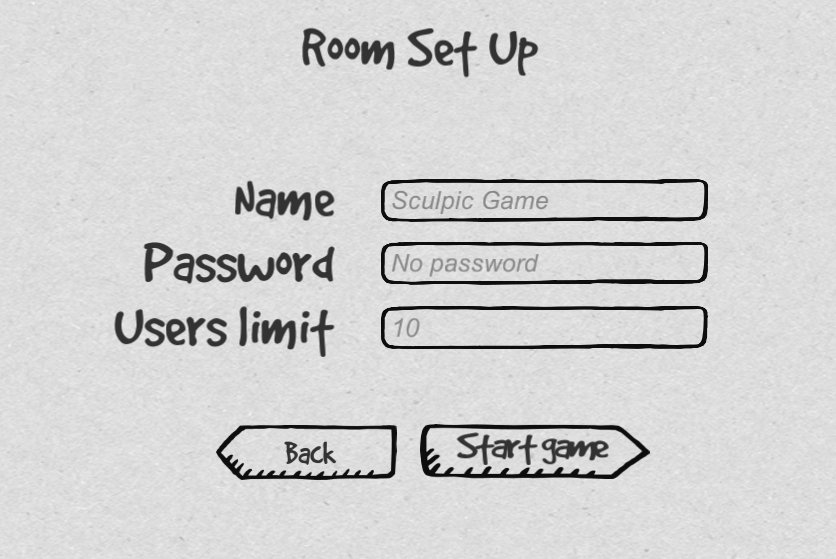
\includegraphics[width=\textwidth]{NewRoom}
\caption{Ekran ustawień nowego pokoju.}
\label{fig:newroom}
\end{figure}

Logika zarządzania pokojami zawarta jest w klasie RoomManager. Zawiera ona listę aktualnie uruchomionych pokojów a jej główną metodą jest metoda CreateNewRoom. Jako iż nie jest możliwe dodanie własnych argumentów uruchomienia programu stworzonego w Unity, przekazanie parametrów pokoju musiało zostać obsłużone w inny sposób:
\begin{enumerate}
\item Tworzony jest nowy katalog, który będzie katalogiem roboczym nowego procesu Unity.
\item W katalogu do pliku XML zapisywane są ustawienia nowego pokoju.
\item Uruchamiany jest proces RoomHoster, który jest wersją aplikacji klienckiej zbudowanej ze sceną RoomHoster. Program ten na starcie odczytuje konfigurację, ustala pierwszy wolny port i automatycznie rozpoczyna hostowanie pokoju.
\end{enumerate}

\subsection{Server Host}
Aplikacja konsolowa służąca do hostowania serwisów jest bardzo prosta – przy starcie uruchamiane są hosty poszczególnych serwisów, naciśnięcie dowolnego klawisza kończyć działanie programu. Najważniejszym elementem aplikacji jest plik konfiguracyjny App.config, który definiuje punkty dostępowe dla serwisów. Typem wiązania używanym przez usługi jest „WebHttpBinding” z racji tego, że są one konsumowane za pomocą zapytań HTTP (architektura REST), a nie przy użyciu wiadomości SOAP.

\begin{figure}[htbp]
\centering
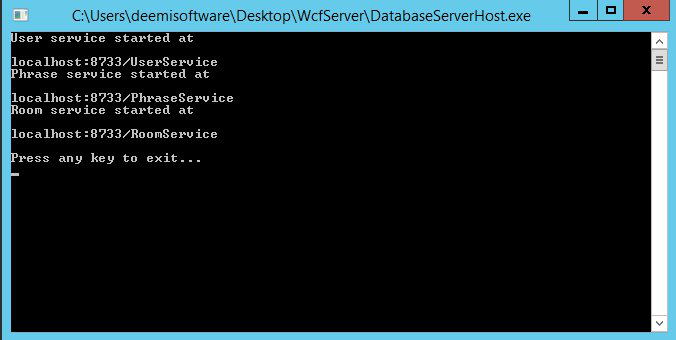
\includegraphics[width=\textwidth]{DatabaseConsole}
\caption{Wygląd uruchomionej aplikacji hostującej serwer bazodanowy.}
\label{fig:databaseconsole}
\end{figure}